\section{Results}
\label{sec:results}
As stated in the introduction, section \ref{sec:intro}, this literature study was complicated by 
the blurring lines between physical, digital, and biological spheres.
This literature study set out to discover the state-of-the-art of research on the energy efficiency impact of, \textbf{explicitly} \textit{robotics software}.
Meaning the explicit impact on energy efficiency of various aspects of the software itself.
It became quickly apparent during the search and selection process, as described in section \ref{sec:study_design:search_selection}, 
that few studies existed on this specific topic.
Out of all 683 potentially relevant studies, only two studies have been found that explicitly research this topic.

One study \cite{rahman2019cloud_robot_offloading} provides proof that a software architectural change; 
from on-board calculations to off-loading to more available robots or the cloud, actually impacts energy efficiency positively.
Another study \cite{hou2017novel_cloud_evaluation_model} presents a novel evaluation technique for cloud robotics, estimating energy efficiency.
The technique allows for identifying those robotics software aspects that consume relatively more energy. 
It can also be used to predict the energy consumption of a specific piece of robotics software, allowing it to be used during software development, 
to create more energy efficient software from the moment it is designed.

The fact that these two studies were the only ones explicitly covering research into the energy efficiency impact of robotics software aspects will
form the basis of the discussion, given in section \ref{sec:discussion}.
To prevent an insignificant literature study, the focus has been shifted from looking at software aspects, to seeing what impact 
robotics software in general can have on energy efficiency. The blurred distinction between software and hardware in robotics made the 
application of the inclusion criteria a tough process.
The final selection of primary studies is the result of a rigorous application of these criteria; 
a study had to explicitly cover \textit{some} software aspect in relation to energy efficiency.

In this section, the insights gained from the data sheet are summarized and given for each column in subsection \ref{sec:results:insights}.
Hereafter, this section is structured according to the research questions.
Each of those subsections gives a detailed explanation of the findings of this literature study in the context of that research question.
The main findings of each research question are presented at the end of each corresponding subsection.

% ========================================================================= Insights =========================================================================

\subsection{Data sheet insights}
\label{sec:results:insights}
The insights, as gained by each of the columns of the data sheet, are given in this subsection.
Any conclusions drawn from these insights in order to answer the research questions targeted by this literature study,
are given in their respective subsections \ref{sec:results:rq1_pub_trends}, \ref{sec:results:rq2_state_of_the_art} and \ref{sec:results:rq3_trade_off}.

\vspace{2mm}

\noindent\textbf{1. Date:}
\begin{figure}[t]
    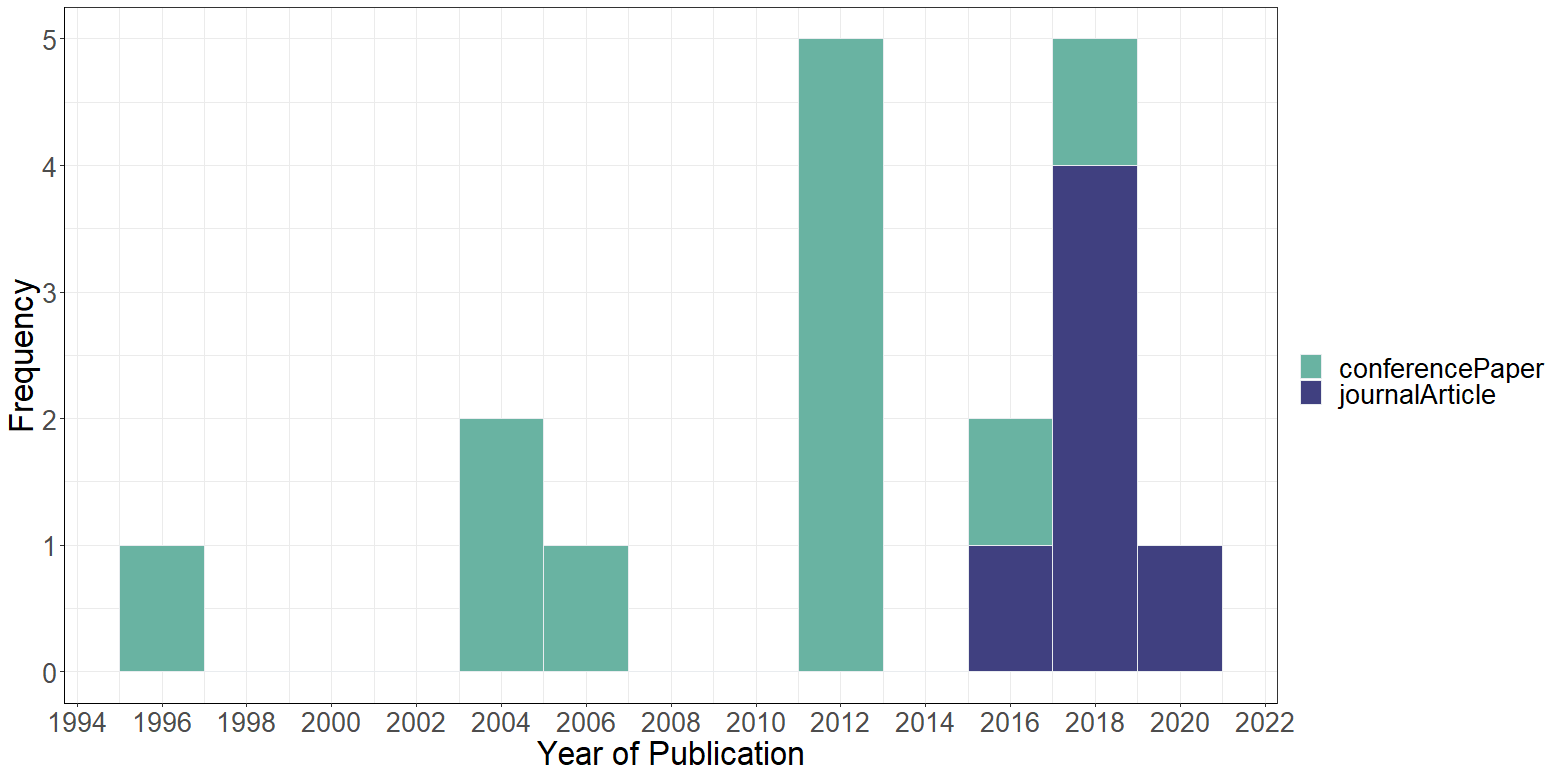
\includegraphics[width=250pt]{figures/publication_trend_extended.png}
    \caption{Publication trends by type}
    \label{fig:pub_trends}
\end{figure}
In figure \ref{fig:pub_trends}, it can be observed that, even though this field of study has been around since before the change of the century,
it truly attained interest in the last decade (2010 - 2020), with a significant spike nearing 2020.
It should also be considered that the 1995 paper is only 3 pages long and discusses the energy impact
of, then novel, on-board motion calculation considering moving obstacles (i.e. people) \cite{barili1995efficient_motion}.
Quite advanced for those times, but nowadays a given.
It can also be observed that the more thoroughly peer reviewed, higher quality research; journal articles are only published in the last $\pm 5$ years.

\vspace{2mm}

\noindent\textbf{2. Metric:} % Might be more sensible to change to Efficiency Metric
% Various metrics used
% Power and Energy separate
% Joules / KiloJoules / NanoJoules most popular.
% Most intersting: FPS / W etc.
% Conclusion: Many different metrics, joules most popular, comparison difficult
It can be observed that the metrics used in the primary studies differ significantly.
In the case that a simplified energy model is used, as explained in part 10 of this subsection, the metric is the most unique;
units of distance traveled per units of energy \cite{mei2006mobile_exploration, patel2012exploration_strategy}.

All other metrics given, use a study specific metric in relation to either; energy, \textbf{Joules} (\textit{J}) or power, \textbf{Watts} (\textit{W}).
The three most common, descriptive and comparable metrics observed are:
\begin{enumerate}
    \item $FPS\footnote{Frame rate (expressed in frames per second or FPS)} / Watt$ \cite{cheng2018FPGA_image_recognition}
    \item $Joules / Meter$ \cite{licea2013wireless_comms}
    \item $Joules / H$ or $Watts / H$ \cite{kim2016firefighting_robot,barili1995efficient_motion}
\end{enumerate}

\vspace{2mm}

\noindent\textbf{3. QA Trade-off:}
% Various trade-offs mentioned.
% Used in RQ 3.
From the 17 primary studies, 15 present a technique to significantly improve energy efficiency.
In each of these studies, a trade-off between the improved energy efficiency and some other attribute(s) of the system can be observed. 
The remaining two studies present techniques to analyze the energy efficiency of a system, and do not present any trade-off with any other
attribute of a system.

\vspace{2mm}

\noindent Each trade-off has been formally mapped to the \textit{Software Quality Attributes\cite{iso2011quality_attributes}}.
However, considering robotics, there are attributes that do not exist in software.
One such attribute has been found to trade-off with Energy Efficiency; Mobility.
Mobility is an attribute paramount to robotics, a system's mobility is
characterized by its ability to respond to its environment 
and the intelligence, speed and the degree to which the response is calculated and executed.
From the primary studies it can be observed that Energy Efficiency trades-off with the following attributes:

\begin{itemize}
    \item Performance Efficiency
    \item Maintainability
    \item Reliability
\end{itemize}

These trade-offs are further detailed; answering the third research question, in subsection \ref{sec:results:rq3_trade_off}.
Considering Mobility, as it is not an official quality attribute 
as described in the referenced literature, it will be discussed informally.

\vspace{2mm}

\noindent\textbf{4. Application Domain:}
% Exploration / Service robots
\begin{figure}[t]
    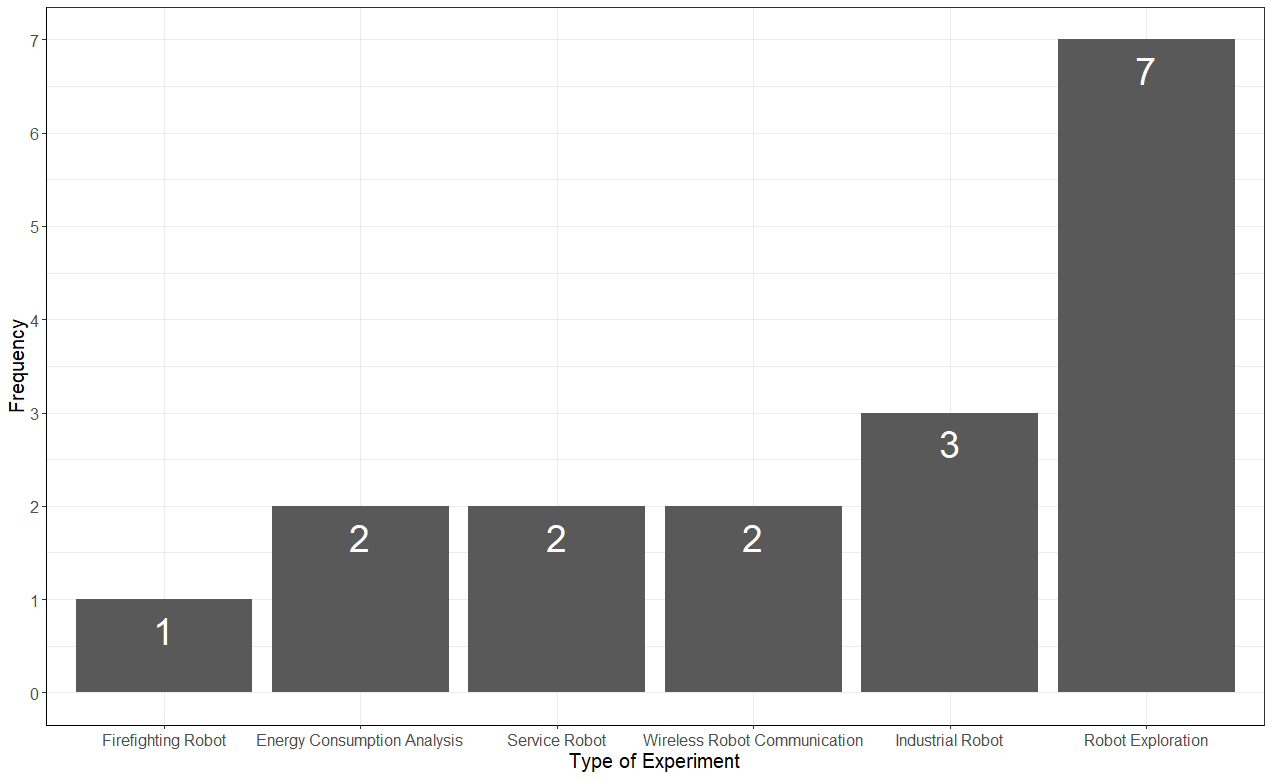
\includegraphics[width=250pt]{figures/domain_freq_barplot.png}
    \caption{Application domains frequency}
    \label{fig:app_domains}
\end{figure}
In figure \ref{fig:app_domains} it can be observed that the application domain of \textbf{Robot Exploration} is the most frequent
domain considered in the primary studies. 
The domain of \textbf{Industrial Robot} is in second place with less than half the frequency.

This is interesting, considering that in terms of emmissions and energy saving potential, there is far more to achieve in the industrial domain
as specified in the introduction; section \ref{sec:intro}.
From this statistic one could thus reason that the combination of functional and efficiency improvements form the main motivation for improving energy efficiency. 
The extension of the operational time of a mobile robot, as a result of the improved energy efficiency, 
is far more functionally relevant than reducing the energy consumption of an industrial robot;
considering the industrial robot has a continuous power supply, energy efficiency is not as functionally important as it will
not deliver any functional improvement.
On the contrary, one could in such a case reason that any improvement of Energy Efficiency decreases Performance Efficiency.
This will be further detailed in subsection \ref{sec:results:rq3_trade_off}.

\vspace{2mm}

\noindent\textbf{5. Identified Major Consumers:}
% Software inefficiencies
% Hardware inefficiencies
% Hardly win-win, only when time reduced, hardware inefficiency reduced etc. (only with software?)
The identified major consumers in the primary studies vary considerably, as can be seen in appendix \ref{appendix:data_sheet_1} and \ref{appendix:data_sheet_2}.
This is a result from the different application domains and their implementation specific details.
However, a common theme can be identified:

No matter the application domain, any identified inefficiency can always be traced back to a (physical) \textit{hardware} inefficiency, 
which is solved by improving \textit{software}.

Considering robots use software to control their hardware, and the fact that robots exist to satisfy some physical need, this is logical.
Within this domain of physical inefficiencies, groups of identified major consumers can be observed.
The observation and formulation of these groups are, of course, subject to personal bias.
This threat to validity has however been mitigated, more about this can be read in section \ref{sec:threats}.
The observed groups consist of the following:

\vspace{2mm} \noindent \textbf{5.1. Movement related:}
Many papers consider the significant energy consumption of robotic movement. 
Especially stops, directional changes, the degree to which the direction is changed and acceleration and decelleration are commonly observed
to contribute significantly to the total energy consumption 
\cite{mei2005energy_consumers_identified, mei2006mobile_exploration, xie2018mecanum_wheel,kaitwanidvilai2020industrial_robot_cycle_time}.

\vspace{2mm} \noindent \textbf{5.2. Inefficient Hardware:}
Inefficient Hardware is commonly identified to be a major consumer. 
This category encapsulates those circumstances where the hardware used is inefficient compared to other solutions 
(e.g. an accelerator for vision-based tracking instead of a more efficient FPGA\footnote{Field Programmable Gate Array} \cite{cheng2018FPGA_image_recognition})
or the hardware is used inefficiently (e.g. loss of traction due to a too heavy payload weight \cite{kim2016firefighting_robot}).

\vspace{2mm} \noindent \textbf{5.3. Inefficient Procedure:}
This group seems to be encapsulating the previous two at first glance. 
However, considering the specificity with which papers focus on one aspect of a system such a paper typically does not take the encapsulating procedure into account.
Using the Oxford definition of a procedure\footnote{\url{https://www.lexico.com/en/definition/procedure}}; a series of actions conducted in a certain order or manner.
This group thus considers identified major consumers where the set of actions conducted in the specified manner would result in an inefficient use of energy.

Some examples would consist of the following:
\begin{itemize}
    \item The use of a traditional DWA local trajectory planner in combination with mecanum robotic wheels \cite{adascalitei2011mecanum_wheels}.
    \item An industrial multi-robot production cell using an inefficient scheduler, resulting in significant idle times \cite{wingstrom2013robot_cell_scheduling}.
    \item Broadcasting data over a wireless connection from a bad position, resulting in a significantly low channel gain and a lossy connection \cite{licea2013wireless_comms}.
\end{itemize}

These examples could all be improved using an improved or, in some cases a completely different, procedure.

\vspace{2mm} \noindent \textbf{Software as consumer:}
From all the primary studies, only one solely identifies software itself as the main consumer \cite{hou2017novel_cloud_evaluation_model}.
It presents a novel cloud evaluation method; which evaluates the energy efficiency of the software itself.
Using the method, the execution of the software itself can be made more efficient. 
The fact that this is the only study addressing this aspect of robotics software, forms the basis of the discussion in section \ref{sec:discussion}.

\vspace{2mm}

\noindent\textbf{6. Identified Improving Software Aspect:}
% Mostly solving hardware with software
Among the primary studies, the identified major consumers are bettered by improving the robotics software;
as this literature study explicitly targets such studies.
As the presented improvements are implementation specific, they are hardly comparable.
However, a common theme among the improvements can be identified:
each improvement solves a hardware inefficiency using software; however, each improvement does so to a varying degree. 
These aspects are processed in the contributions of each primary study, 
as stated in the next part (7) of this subsection.

Groups can be observed among the identified improving aspects.
As the improving aspects are cohering with the observed major consumers, as they aim to improve them,
the groups are inherently related.
The observed groups consist of the following:

\vspace{2mm} \noindent \textbf{6.1. Improved Hardware:}
Those systems and applications where the used hardware can be considered inefficient, 
either in its use for that specific application (i.e. the accelerator vs FPGA),
or its use in general (i.e. the loss of traction due to a too heavy payload weight)
can be improved in terms of energy efficiency by improving the used hardware.
Some examples of improving the system's hardware, consequently improving its energy efficiency consist of:
\begin{itemize}
    \item Off-loading computations from on-board hardware to more energy optimized, better utilized cloud infrastructure \cite{rahman2019cloud_robot_offloading}.
    \item The use of an FPGA for vision-based tracking instead of the common accelerator \cite{cheng2018FPGA_image_recognition}.
    \item Adding sub-robots to a system to distribute payload weight and prevent energy inefficient use of hardware \cite{kim2016firefighting_robot}.
\end{itemize}

For each of these examples, as observed in the primary studies, the betterment of energy efficiency has been proven, evaluated and tested
as the selection criteria for making it into the primary study set demands so.

\vspace{2mm} \noindent \textbf{6.2. Improved Procedure:}
As described before, the procedure - a series of actions conducted in a certain order or manner - can be a source of inefficiency in terms of energy.
Therefore improving these procedures can lead to conducting these actions more energy efficiently.
Some examples of improving procedures to improve energy efficiency consist of:
\begin{itemize}
    \item Improving algorithms related to robotic motion to reduce stops, turns and moments of acceleration or decelleration by improving either the path planning itself
    or the obstacle avoidance algorithm. Resulting in more energy efficient motion 
    \cite{xie2018mecanum_wheel,mei2006mobile_exploration, mei2005energy_consumers_identified, barili1995efficient_motion, jia2004grid_strategy_exploration, kaitwanidvilai2020industrial_robot_cycle_time}.
    \item Reducing the idle time of robotic systems by improving the procedures responsible for task distribution and execution 
    \cite{kaitwanidvilai2020industrial_robot_cycle_time, gurel2019industrial_robot_scheduling, wingstrom2013robot_cell_scheduling}.
    \item Making a robotic system able to predict the energy cost of stimuli and base the decision to act on it on the available energy budget \cite{kirtay2013humanoid_emotion}.
\end{itemize}

It should be noted that although a clear relation can be seen between the groups observed for major consumers and improving aspects, 
a movement related specific group is missing for identified improved aspects.
The simple reason that this is the case, is the fact that improving movement related aspects inherently requires either 
an improved procedure for planning that movement, improved hardware that consumes less energy for the same amount of movement
or a combination thereof.

\vspace{2mm}

\noindent\textbf{7. Major Contribution:}
% For example the entire system, integrating the software aspects to improve inefficiency.
For each of the primary studies the major contribution is the implementation and evaluation of the identified software aspect that would
improve the energy inefficiency. 
This column can therefore be seen as an extension of the previous column; part 6 of this subsection.
These contributions are further detailed; answering the second research question, in subsection \ref{sec:results:rq2_state_of_the_art}.
Grouping these contributions would largely overlap with the groupings for the previous two grouped metrics, and is therefore a redundant activity.

\vspace{2mm}

\noindent\textbf{8. Experiment:}
% Experiment performed most common: simulation, why?
\begin{figure}
    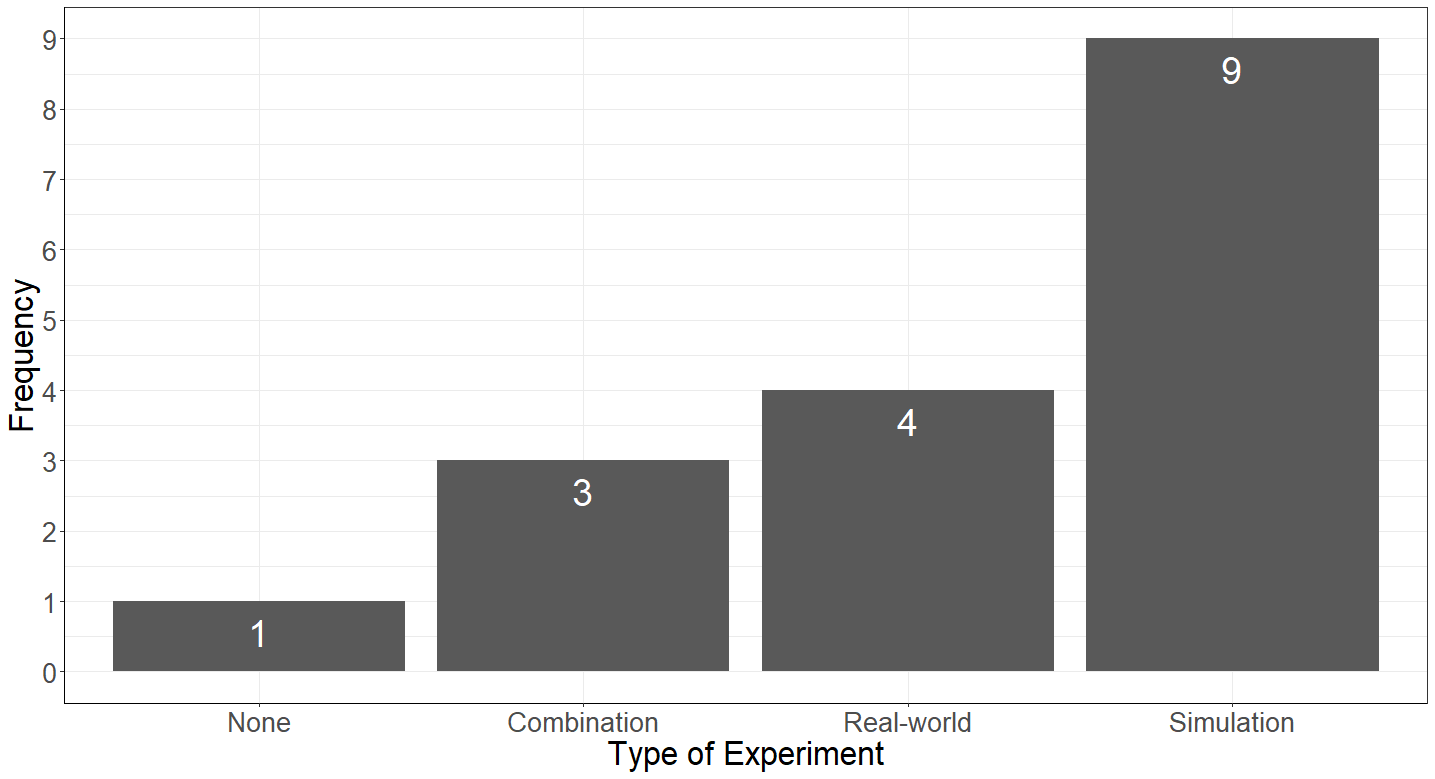
\includegraphics[width=250pt]{figures/exp_freq_barplot.png}
    \caption{Experiment distribution}
    \label{fig:experiment_distr}
\end{figure}
From figure \ref{fig:experiment_distr}, it can be observed that most studies performed an experiment, only one primary study did not.
It can be observed that most studies, 9 out of 17, perform an experiment in the form of a simulation, 
this is without counting the combination of real-world and simulation.
Considering those; 12 out of 17 primary studies used a simulation as an experiment.
Out of the primary studies, 4 studies performed a real-world experiment and 3 performed a combination of real-world and simulated experiments.

\vspace{2mm}

\noindent\textbf{9. Comparison Against State-Of-The-Art:}
% Mostly yes, important for validity!
To verify the validity of the claims presented in the primary studies, the comparison against the state-of-the-art is important.
In 14 of the 17 primary studies a comparison was made.
From the three studies that had no comparison, one was a paper presenting a novel cloud evaluation method \cite{hou2017novel_cloud_evaluation_model}
which has no state-of-the-art to compare to as it presents something novel. 
It can thus be safely concluded that 15 of the 17 primary studies uphold the comparison.
This is of importance as this literature study's validity is dependent upon the validity of the literature it is based on.

The most notable comparisons against the state-of-the-art, as observed in the literature, consist of the following.
The specific results compared to the state-of-the-art for each paper are 
purposefully omitted to prevent any erroneous comparisons between the papers and their results.
Each of the results should be considerd on their own, 
compared to the relative state-of-the-art, and for such nuance, 
one should read the referenced literature.

\vspace{2mm} \noindent \textbf{9.1. Exploration algorithm.}
The state-of-the-art with respect to exploration algorithms for mobile robots
consisted of selecting the next target for exploration based on the utility - amount of area to be explored - 
and the cost - the distance of the target to the current position - of the frontier cell 
\cite{burgard2005multi_robot_exploration, simmons2000multi_robot_exploration,zlot2002multi_robot_exploration}.
In the studied literature it is however proven that if the next target is selected based on the orientation of the robot,
overlap in the robot trajectory is guaranteed to be impossible \cite{mei2006mobile_exploration}.
Reducing energy consumption, and reducing total travel distance; enabling the mobile robot 
to finish exploring the area faster while consuming less energy. 

\vspace{2mm} \noindent \textbf{9.2. Energy efficient macanum motion control.}
Mecanum wheels are the state-of-the-art in industry when it comes to omnidirectional wheel designs with a high load capacity \cite{xie2018mecanum_wheel}.
The Ilon Mecanum wheel is one of the practical omnidirectional wheel designs utilized in the industry, 
and it has the advantage of high load capacity over other omnidirectional wheel designs \cite{adascalitei2011mecanum_wheels}.
However, the Mecanum wheel trades off maneuverability against motion efficiency, and its inefficient energy usage for generating omnidirectional 
motions increases the energy consumption of the robot \cite{diegel2002improved_mecanum_wheel}.
The study extends the popular, well-known, robot operating system (ROS) dynamic window approach (DWA),
a reactive collision avoidance navigation concept \cite{fox1997dwa_paper}.
DWA has proven performance over a range of extended applications \cite{brock1999dwa_usage_1,ogren2005dwa_usage_2,kiss2012dwa_usage_3}.
The study added energy-related criterion to the DWA local trajectory planner,
which proved to minimize energy consumption per dynamic window.

\vspace{2mm} \noindent \textbf{9.3. Energy efficient, multi-robot firefighting}
To lessen the deaths \cite{fahy2015firefighter_deaths} and property damages \cite{karter2013fire_damages} 
caused by fires in the United States, many researchers have studied various kinds of solutions. 
One of the most effective solutions is using a firefighting robot that can 
substitute for firefighters on the fire scene. This state-of-the-art solution
is however often implemented as a single robot (e.g. FIRO-M), 
carrying a heavy hose full of water into the fire scene.
The robot often suffers from a loss of traction because the hose full of water
is too heavy, or the hose gets stuck on a corner the robot has just driven around \cite{kim2016firefighting_robot}.
To get unstuck, the robot will have to drive back and forth. 
Both consume significant amounts of energy that is not used for fighting the actual fire.
To address this, the study presents MRESS - multi-robot energy saving system - to increase
the operating time of a firefighting robot.
The addition of sub-robots, aiding in carrying the hose, 
allow for a better weight distribution, preventing a loss of traction, 
and the advanced vision-based fire hose tracking method prevents 
that the hose gets stuck on corners.
Compared to the state-of-the-art, the single firefighting robot, 
this saves significant amounts of energy and allows for a longer operating time.

\vspace{2mm}

\noindent\textbf{10. Energy Model:}
% Interesting for future research / comparison between the relative studies
The energy model used is given for each of the primary studies in appendix \ref{appendix:data_sheet_2}.
The validity of the contributions of the studies is dependent on the validity of the energy model used (if applicable), 
these are therefore recorded. 
They can also be valuable for any practitioner or researcher that seeks insight into energy models for robotics simulation.

Many different energy models have been used by the various primary studies, some try to simulate the energy consumption 
as precisely as possible by simulating drag, torque, acceleration, decelleration, etc. with extensive mathematics and physics equations. 
These models are called \textit{representational}.

Opposite from representational models, is the \textit{abstract} model. 
This model is used in cases where representational simulation is not necessary, 
and only the relevant difference in energy consumption between that which is researched is of importance.
These models can therefore be simple in their nature.

\vspace{2mm} \noindent \textbf{Energy model shortcoming:}
An interesting observation can be made from studying the various energy models present in the studied literature; 
none of the energy models are capable of simulating any computational energy usage.
Therefore, in studies where this is of importance, only a real-world experiment was able to provide these insights.

\vspace{2mm} \noindent \textbf{10.1. Abstract Simple Model}
The abstract simple model is relevant in use cases where only differences in relevance to one another of that which is researched is of importance.
The gathered metrics will be in no way representational and comparable to the real world, 
but can be used to simply and clearly depict differences with relative credibility.
Espcially when coupled with results from a real-world experiment, as can be often seen in studies that use such models.

An example of an abstract simple model would consist of the following:

Two papers use the same approach as their energy model, which can be identified as an abstract simple model.
It is the only model among the primary studies which is used by multiple papers;
these papers are written by different authors but within the same field of study; mobile robot exploration.
The model they use consists of a simulated grid, where each grid cell consists of 1x1 Units of Distance, 
and travelling 1 Unit of Distance equals 1 Unit of Energy.
Each stop costs 0.5 Units of Energy and each 45° turn costs 0.4 Units of Energy, each additional 45° adding another 
0.2 Units of Energy to the total cost.
Meaning: a 90° turn would cost 0.6 Units of Energy and a 135° turn would cost 0.8 Units of Energy etc.

\vspace{2mm} \noindent \textbf{10.2. Representational Complex Model}
Representational energy models are models that can be used in simulations where results would need to be comparable to the real-world.
These models are often complex of nature and require extensive information about the robotic system considered, such as
friction coefficients (e.g. rolling, sliding and viscous), wheel radius, robot mass, static friction torgue, 
idling power consumption, gear ratio etc.
This information is then to be used in accurate physics equations that are capable of modeling the robotic system accurately and
representational to the real-world.

Mathematics and kinematics\footnote{\url{https://www.lexico.com/en/definition/kinematics}} 
- the branch of mechanics concerned with the motion of objects without reference to the forces which cause the motion -
are extensively used in these models to get results as close to the real-world as possible.

% ========================================================================= RQ 1 =========================================================================

\subsection{Results - publication trends (RQ1)}
\label{sec:results:rq1_pub_trends}

In this section the results obtained when analyzing the publication trends on energy efficiency in robotics software are presented.
Understanding the publication trends in the field of study is essential for interpreting the results of this literature study as it gives
an idea of the maturity of the field. 

\vspace{2mm}

From these findings, as stated in part 1 of subsection \ref{sec:results:insights}, we can conclude that the maturity of the field is rather limited,
considering the number of publications decrease significantly the further back we go in time.

\vspace{2mm}

It is important to take this into account for the findings of this literature study, presented in the following subsections 
\ref{sec:results:rq2_state_of_the_art} and \ref{sec:results:rq3_trade_off}, and for the discussion as presented in section \ref{sec:discussion}.
Considering the aforementioned difficulty with the initial goal of this literature study; from the publication trends we can see that this 
is probably the case because of a rather immature field of study.

\vspace{2mm}

\noindent\fcolorbox{black}[HTML]{FFFFFF}{\parbox{0.47\textwidth}{%
\noindent \textbf{Main Findings.}
\begin{enumerate}[nolistsep]
\item The field of study has been around since before the change of the century.
\item The field can still be considerd immature as publications only recently attained in numbers.
\end{enumerate}}}

% ========================================================================= RQ 2 =========================================================================

\subsection{Results - state-of-the-art (RQ2)}
\label{sec:results:rq2_state_of_the_art}
In this section the state-of-the-art in analyzing and improving energy efficiency in robotics software is presented as found from studying the primary studies.

\vspace{2mm}

\noindent\textbf{1. Analyzing:}
The novel cloud evaluation method \cite{hou2017novel_cloud_evaluation_model}, introduces a whole new paradigm in robotics software.
This can be concluded as it is the only paper out of 683 potentially relevant studies, and 17 primary studies, 
that explicitly looks at the execution of robotics software itself for improvement of energy efficiency.

It presents a novel method to evaluate the energy efficiency of a specific piece of software.
The method can be used on existing software, to identifiy bottlenecks, or used during the development of the software itself;
providing the ability to improve the energy efficiency of the software execution during design time.

It can be considered the state-of-the-art of evaluation and analysis, in robotics software.
However, it should be considered that this was the only paper that focussed so explicitly on software and its impact on energy.
Considering the 16 other primary studies, and the observations made as stated in part 8 of subsection \ref{sec:results:insights}; 
it can be stated that another big standard in this field is the evaluation through practice; 
in the form of a simulation, a real-world experiment or a combination thereof.

\vspace{2mm}

\noindent\textbf{2. Improving:}
The techniques to improve energy efficiency in robotics software vary significantly across the primary studies. 
As stated in part 5 and 6 of subsection \ref{sec:results:insights}; a trend observed is that they mostly solve hardware (physical) 
inefficiencies using software solutions, like an improved algorithm.

As stated before, this literature study initially set out to research the state-of-the-art in terms of improving the
energy efficiency of robotics software \textit{itself}.
The fact that only two of the primary studies presented such research forms the basis of the discussion in section \ref{sec:discussion}. 
This section will therefore detail what has been found by studying the primary studies in the context of improving energy efficiency 
by \textit{using} robotics software.
Each primary study presented an evaluated software solution that improves energy efficiency.
The techniques extracted from the primary studies consist of:

\vspace{1mm}

\textbf{1 Off-loading computations.} The technique to off-load computations to other, nearby, robots that are more 'available' 
(i.e. robots that have more resources available for such computations relative to the current one.), or to off-load it to the cloud.
The concept here is that the cloud infrastructure (hardware itself, hardware utilization, etc) is more energy-optimized compared to the
hardware used on the robots themselves, and will thus result in an improved energy efficiency.
Even though some energy is wasted in the transmission of data, the overall energy consumption is decreased \cite{rahman2019cloud_robot_offloading}.
    
\vspace{1mm}

\textbf{2 Advanced motion algorithm.} The technique to improve the motion algorithm, such as path finding algorithms for mobile robot exploration. 
The improvement involves incorporating techniques to facilitate energy efficient movement.
Techniques like \textbf{3, 4 and 5} can be implemented in an advanced motion algorithm.
Like implementing a more advanced obstace-avoidance algorithm, enabling the robot to steer less by steering earlier to avoid the obstacle \cite{xie2018mecanum_wheel}.
Also, many existing studies select the next target based on the utility and cost of the frontier cells 
\cite{burgard2005multi_robot_exploration, simmons2000multi_robot_exploration,zlot2002multi_robot_exploration} 
However, study \cite{mei2006mobile_exploration} proves that if the next target is selected based on the orientation of the robot, 
overlap in the robot trajectory is guaranteed to be impossible; reducing energy consumption and reducing the total travel distance.
Enabling the mobile robot to finish exploring the area faster while consuming less energy.
    
\vspace{1mm}

\textbf{3 Limiting motion changes.} The technique to limit stops, directional changes (turns) and the degree to which the direction is changed as much as possible 
significantly improves energy efficiency. By the very nature of this technique, an improved obstacle detection and avoidance algorithm
is needed for mobile robotic systems
\cite{xie2018mecanum_wheel, kim2016firefighting_robot, benkrid2016multi_robot_exploration, barili1995efficient_motion, 
jia2004grid_strategy_exploration, mei2005energy_consumers_identified, patel2012exploration_strategy}.
    
\vspace{1mm}

\textbf{4 Limiting motion speed.} The technique to limit motion at high speeds, with numerous moments of acceleration and decelleration
\cite{wingstrom2013robot_cell_scheduling}.
    
\vspace{1mm}

\textbf{5 Limiting idle time.} The technique to prevent idle time as much as possible \cite{gurel2019industrial_robot_scheduling, 
kaitwanidvilai2020industrial_robot_cycle_time, wingstrom2013robot_cell_scheduling}.
    
\vspace{1mm}

\textbf{6 Limiting unnecessary communication.} The technique to limit data transmission by preventing the transmission of duplicate 
or otherwise unnecessary data in multi-robotic systems \cite{huh2013distributed_swarm}.

\vspace{1mm}

\textbf{7 Limiting physical inefficiencies.} The technique to limit physical inefficiencies (e.g. loss of traction because of payload weight), if possible, by adding more robots to the system which would cause the overall
energy consumption to go down as the loss of traction was consuming more energy than the addition of the subrobots \cite{kim2016firefighting_robot}.
    
\vspace{1mm}

\textbf{8 Using optimized hardware.} The technique to use more advanced hardware (i.e. more energy-optimized, desktop grade, hardware instead of custom robotic hardware) 
on robots in combination with energy-optimized software \cite{cheng2018FPGA_image_recognition}.
    
\vspace{1mm}

\textbf{9 Limiting transmission loss.} The technique that sacrificing some energy on finding a better position for the transmission of data over a wireless connection,
to increase higher channel gain, will ultimately improve energy efficiency as less time is spend and wasted on (re)transmitting 
data over a lossy wireless connection \cite{licea2013wireless_comms}.

\vspace{1mm}

\textbf{10 Predicting task's energy cost.} The technique to be able to predict the energy cost of any stimuli and reject said stimuli if it is predicted to exceed some energy threshold 
\cite{kirtay2013humanoid_emotion}.

\vspace{2mm}

\noindent\fcolorbox{black}[HTML]{FFFFFF}{\parbox{0.47\textwidth}{%
\noindent \textbf{Main Findings.}
\begin{enumerate}[nolistsep]
\item The state-of-the-art on analyzing the energy efficiency of robotics software consists of evaluation techniques capable of
estimating the energy efficiency of a piece of robotics software and identifying energy efficiency bottlenecks in existing robotics software.
\item The most common way to analyze the energy efficiency of robotics software consists of performing experiments, evaluating the results.
\item The state-of-the-art on improving the energy efficiency consists of:
    \begin{enumerate}
        \item Off-loading computations to more energy-optimized infrastructure.
        \item Improved path finding, obstacle avoidance etc.
        \item Limit physical inefficiencies, idle time, acceleration, decelleration, stops, turns, directional changes and the extent of the directional change.
        \item The use of more energy-optimized hardware on robotics themselves.
        \item Sacrificing some energy to achieve higher efficiency (e.g. finding a better location with better signal for data transmission).
        \item Using elaborate software to be able to predict the energy cost of stimuli and reject if necessary.
    \end{enumerate}
\end{enumerate}}}

% ========================================================================= RQ 3 =========================================================================

\subsection{Results - QA trade-off (RQ3)}
\label{sec:results:rq3_trade_off}
From the primary studies, it can be observed that most techniques that significantly improve energy efficiency come with a cost to some other attribute of the system.
As stated in part 3 of the subsection \ref{sec:results:insights}, the attributes have been mapped to \textit{Software Quality Attributes\cite{iso2011quality_attributes}}
if possible.

In figure \ref{fig:trade_off_freq} it can be observed that the \textbf{Performance Efficiency} is the most common QA trade-off with 8 occurrences in the 17 primary studies.

\vspace{1mm}

- \textbf{Performance Efficiency} trades-off with Energy Effiency in any case where physical or software inefficiencies cannot be improved or do not exist. 
Techniques that are similar to techniques \textbf{3, 4, 5 and 9} from subsection \ref{sec:results:rq2_state_of_the_art}, 
will inherently decrease Performance Efficiency as it is the only way such techniques improve Energy Efficiency.

It should be noted that some techniques, similar to techniques \textbf{1, 2, 6, 7 and 8}, both improve the Performance Efficiency and Energy Efficiency. 
It has been observed that this is often the case using techniques that will improve a given physical or software inefficiency. 
For example, technique \textbf{2} improves the path planning algorithm, guaranteeing \textit{no path overlap} during area exploration. 
It has been proven that this not only improves Energy Efficiency, but also allows the robot to explore the unknown area faster; 
thus improving Performance Efficiency \cite{mei2006mobile_exploration}.

\vspace{1mm}

\begin{figure}[t]
    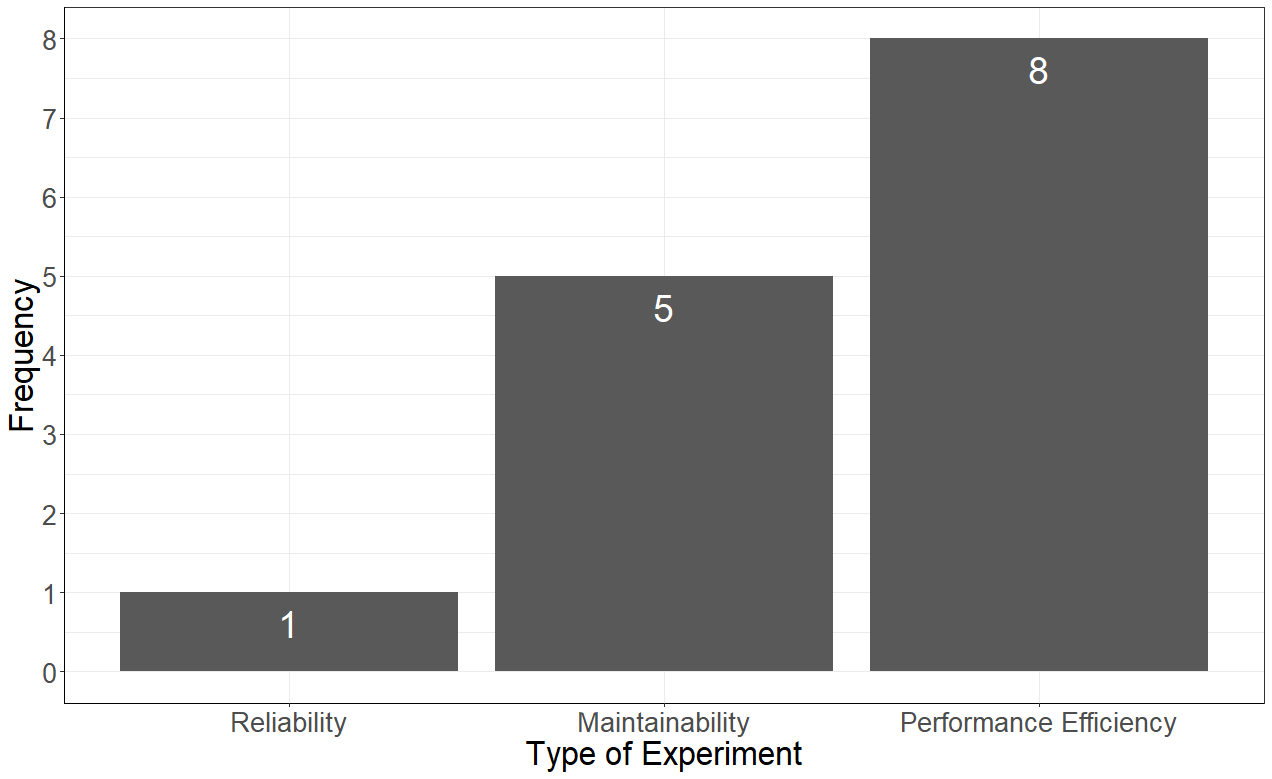
\includegraphics[width=250pt]{figures/tradeoff_freq_barplot.png}
    \caption{QA Trade-off frequency distribution}
    \label{fig:trade_off_freq}
\end{figure}

- \textbf{Maintainability} trades-off with Energy Efficiency in any case where improving Energy Efficiency requires more elaborate and complex software and/or hardware. 
This is the case for each of the observed techniques, to varying degree, as presented in subsection \ref{sec:results:rq2_state_of_the_art}; \textbf{1 - 10}.

\vspace{1mm}

- \textbf{Reliability} trades-off with Energy Efficiency in any case where improving Energy Efficiency requires the system to 
stop operating for some criteria, like using techniques similar to \textbf{10}, or where the chance of operational failure is increased, 
like increasing the possible points of failure during operation using techniques similar to \textbf{1, 7 and 9}. 

Besides the fact that certain QAs need to be traded-off in order to improve energy efficiency, the extent to which this is required 
matters just as much, if not more.
For each system, the hit to the traded-off QA and the improvement of Energy Efficiency will be significantly different.
Thus, an indication of expected results cannot be given.
However, one could reason that a disproportional hit to the traded-off QA, relative to the increase in Energy Efficiency might not be worthwile.

Study \cite{kaitwanidvilai2020industrial_robot_cycle_time} for example states: 

\noindent\textit{"This method reduces energy consumption from 8155.20 to 7148.6 J, 
a decrease of 12.3\%. On the other hand, the total moving time is increased by 71.8\% from 6.60 to 11.34 s".}

In case the system in question can suffer a 71.8\% reduction in Performance Efficiency for a 12.3\% increase in Energy Efficiency, it might be worthwile.
However, it can be considered a good example of a trade-off which might not be worthwile for most systems, let alone time-critical systems.

\vspace{1mm}

\noindent \textbf{Informal attribute discussion}
\newline
\textbf{Mobility} is a quality attribute paramount to robotic systems, 
as robotic systems result from a need to manipulate some environment using hardware, controlled by software.
A system's Mobility is characterized as its ability to respond to its environment and 
the intelligence, speed and the degree to which the response is calculated and executed.
However, Mobility is not referenced as a quality attribute in the official literature and is thus discussed informally.

Mobility trades-off with Energy Efficiency in any case where improving Energy Efficiency requires the system to reduce its responsiveness to 
the environment it exists in. This is the case for techniques where the robot has to limit its movement, techniques similar to \textbf{3 and 4}.

\vspace{2mm}

\noindent\fcolorbox{black}[HTML]{FFFFFF}{\parbox{0.47\textwidth}{%
\noindent \textbf{Main Findings.}
\begin{enumerate}[nolistsep]
\item The most common QA trade-off in order to improve Energy Efficiency is \textbf{Performance Efficiency}.
\item Some techniques will improve both Energy Efficiency and \textbf{Performance Efficiency} at the same time, 
these techniques mostly consist of techniques solving physical and/or software inefficiencies.
Like techniques similar to \textbf{1, 2, 6, 7 and 8}.
\item Each QA trade-off will have a varying degree of impact for each specific system. 
It is up to the reader to decide if such trade-offs are worth it for their system.
\end{enumerate}}}
